\documentclass[a4paper,10pt]{article}
\usepackage{fontspec}
\setmainfont{Times New Roman} % Hoặc chọn font hỗ trợ tiếng Việt
\usepackage[left=1.5cm, right=1.5cm, top=2cm, bottom=2cm]{geometry}
\usepackage{enumitem}
\usepackage{titlesec}
\usepackage{xcolor}
\usepackage{hyperref}
\usepackage{graphicx}
\usepackage{tabularx}
\usepackage{ulem}
\usepackage{booktabs}
\usepackage{fontawesome5} % Thư viện icon
\usepackage{longtable} % Thêm vào phần preamble


\titleformat{\section}{\Large\bfseries\color{black}}{}{0em}{}
\titleformat{\subsection}{\bfseries}{}{0em}{}

\begin{document}
\raggedbottom
\titlespacing{\section}{0pt}{6pt}{3pt}
\titlespacing{\subsection}{0pt}{4pt}{2pt}
% \flushbottom

\noindent
\begin{tabular}{m{3cm} l}
    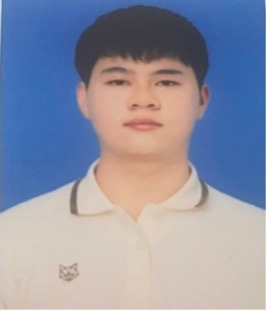
\includegraphics[width=3cm, height=3.5cm]{anh_CV.jpg} &
    % Chia thành 2 cột với 3 dòng mỗi cột
    \begin{tabular}{@{}l}
        \multicolumn{1}{c}{\textbf{\LARGE Nguyễn Hữu Lộc} \quad \textbf{\large Backend Developer Intern}} \\[10pt]
        \begin{tabular}{@{}ll@{}}
            \faEnvelope & \href{mailto:lockbkbang@gmail.com}{\uline{lockbkbang@gmail.com}} \\
            \faPhone & 0397845443 \\
            \faMapMarker & Thoi Tam Thon, Hoc Mon, TP HCM \\
        \end{tabular} 
        \hspace{20pt} % Tạo khoảng cách giữa 2 bảng (cột)
        \begin{tabular}{@{}ll@{}}
            \faFacebook & \href{https://fb.com/huuloc.nguyen.23092004}{\uline{fb.com/huuloc.nguyen.23092004}} \\
            \faGithub & \href{https://github.com/LocNguyenSGU}{\uline{github.com/LocNguyenSGU}} \\
            \faGlobe & \href{https://locnguyensgu.github.io/nguyenhuuloc2k4/}{\uline{my.website}} \\
        \end{tabular} 
    \end{tabular}
\end{tabular}


\section{About me}
\vspace{-10pt}
\noindent\rule{\linewidth}{0.5pt}

Motivated Java Backend Developer Intern with hands-on experience building scalable web applications using Spring Boot. Familiar with RESTful API design and relational databases (MySQL), and have worked with NoSQL databases such as MongoDB. Experienced in implementing authentication and authorization using Spring Security and JWT. Exposure to microservices architecture and real-time communication using WebSocket. Passionate about clean code, eager to learn, and always open to solving new backend challenges. GPA 8.0/10.

\section{Education}
\vspace{-10pt}
\noindent\rule{\linewidth}{0.5pt} % Đường gạch nhẹ
\vspace{5pt}
\begin{tabularx}{\linewidth}{l X}
    \textbf{2022 - 2026} & 
    \textbf{Sai Gon University} \\ 
    & Information Technology, majoring in Software Engineering \\ 
    & GPA: 3.25 \quad \textbf \quad Score: 8.0/10 \\ 
    & Scholarship: 3 times \textit{(Merit-based Encouragement Scholarship)}
\end{tabularx}

\section{Skills}
\vspace{-10pt}
\noindent\rule{\linewidth}{0.5pt} % Đường gạch nhẹ
% Tạo bảng với 3 cột
% Sử dụng tabularx để tự động điều chỉnh chiều rộng cột
\renewcommand{\arraystretch}{1.2}
\begin{tabularx}{\linewidth}{X X X} 
    \textbf{Database} & \textbf{Languages} & \textbf{English} \\
    MySQL, Redis, MongoDB & Java, JavaScript & IELTS 5.0 (practice test) \\

    \textbf{Version Control} & \textbf{Backend} & \textbf{Frontend (basic)} \\
    Git/GitHub & Spring Boot, Servlet, REST API, WebSocket, Microservices (exposure) & ReactJS, JSP \\

    \textbf{Tools} & \textbf{Security \& Integration} & \\
    Docker, Swagger, Git, Clean Code & Spring Security, JWT, Paypal API & \\
\end{tabularx}

\section*{Achievements}
\vspace{-10pt}
\noindent\rule{\linewidth}{0.5pt} % Đường gạch nhẹ
\begin{itemize}
    \item \textbf{Hackathon 2025 (Top 2) - Sai Gon University}: Built an AI-powered learning assistant using OpenAI APIs, integrated into a web platform. Led backend development, applied problem-solving skills and rapid prototyping to deliver a working demo in 24 hours. \href{https://github.com/LocNguyenSGU/Hackathon_Luong_Nghin_Do}{\uline{GitHub Repository}}
\end{itemize}

\section{Projects}
\vspace{-10pt}
\noindent\rule{\linewidth}{0.5pt} % Đường gạch nhẹ

\renewcommand{\arraystretch}{1.2}
\begin{tabularx}{\linewidth}{@{}p{3cm} p{4.5cm} @{ }X}
    \textbf{12/2024 - Present} & \textbf{Calligo} & \\
    & \textbf{Description:} & A real-time messaging and calling platform built using a microservices architecture. It supports instant messaging, voice/video calls, and real-time notifications. \\
    & \textbf{Members:} & 1 member \\
    & \textbf{My roles:} & Designed and implemented the entire system, covering database architecture, backend logic, and frontend UI/UX. Managed authentication, WebSocket-based real-time communication, message storage. \\
    & \textbf{Technology:} & \\
    & \quad \textbf{Database:} & MongoDB, Redis, MySQL \\
    & \quad \textbf{Backend:} & Spring Boot, Kafka, WebSocket, JWT, Microservices Architecture, Observe pattern \\
    & \quad \textbf{Frontend:} & ReactJS, Ant Design \\
    & \textbf{GitHub:} & \href{https://github.com/LocNguyenSGU/Calligo}{\uline{Backend Repository}} \\
    &  & \href{https://github.com/LocNguyenSGU/Calligo-FE}{\uline{Frontend Repository}} \\
\end{tabularx}


\renewcommand{\arraystretch}{1.2}
\begin{tabularx}{\linewidth}{@{}p{3cm} p{4.5cm} @{ }X}
    \textbf{10/2024 - 12/2024} & \textbf{Flight Management System} & \\
    & \textbf{Description:} & Website for managing flight bookings, with features like easy ticket booking, email notifications, VNPAY payments, flight management, comments, Excel report generation, and secure role-based access control. \\
    & \textbf{Members:} & 7 members \\
    & \textbf{My roles:} & Designed the database, set up the backend framework, and implemented core features such as user authentication (login/register/forgot password) using Spring Security and JWT. Developed email notification functionality, Excel export, RBAC, and API documentation with Swagger. \\
    & \textbf{Technology:} & Spring Boot, MySQL, ReactJS, Ant Design, Docker, Swagger \\
    & \textbf{GitHub:} & \href{https://github.com/kietsocola/FlightManagementSystem}{\uline{Backend Repository}} \\
    &  & \href{https://github.com/duylam15/react-flight-management-system}{\uline{Frontend Repository}} \\
\end{tabularx}

\renewcommand{\arraystretch}{1.2}
\begin{tabularx}{\linewidth}{@{}p{3cm} p{4.5cm} @{ }X}
    \textbf{2/2024 - 5/2024} & \textbf{SGU Test} & \\
    & \textbf{Description} & A comprehensive quiz management platform designed for teachers and students. Teachers can effortlessly create quizzes, monitor student performance, and import/export questions easily. \\
    & \textbf{Members} & 4 members \\
    & \textbf{My roles} & Developed a dynamic question creation feature, implemented Excel question importing, handled CRUD operations, designed statistical visualization with Chart.js, and created a landing page with animations. \\
    & \textbf{Technology} & Servlet, JSP, MySQL, HTML, CSS \\
    & \textbf{GitHub} & \href{https://github.com/LocNguyenSGU/SGU-Test}{\uline{Github Repository}} \\
\end{tabularx}


\end{document}
